\chapter{Hyper-Heuristics}\label{chap:hhs}

\begin{quotation}
      ``The capacity to learn is a gift; the ability to learn is a skill; the willingness to learn is a choice.''
\end{quotation}
\begin{flushright}
      - Brian Herbert
\end{flushright}

Chapter \ref{chap:heuristics} introduced the concept of a \index{heuristic}heuristic as an optimisation algorithm that is used in a search process that seeks out optimal solutions to an optimisation problem. Finding the best \index{heuristic}heuristic to use for a given optimisation problem is non-trivial. Furthermore, finding optimal solutions is often dependent on using the appropriate configurations. In the context of training \acp{FFNN}, these configurations could include \index{heuristic}heuristic hyper-parameters and model architecture. It is often the case that the application of a specific configuration only applies to a specific problem and does not necessarily translate or generalise to other problems~\cite{ref:kheiri:2017}.

The optimal configuration of \index{heuristic}heuristics to use, along with hyper-parameters and model architecture, lies in some hyper-dimensional \textit{configuration space} yielding yet again, another optimisation problem on its own. Traditionally, if multiple configurations are to be considered, an empirical process of trial and error is executed. Trial and error approaches are time consuming and laborious.

One particular approach to the configuration optimisation problem mentioned above, is to try and automate the process to find the best configuration. One such automated process involves considering many different configurations in an iterative fashion, sweeping over different configurations parameters within the configuration space. Techniques such as \acf{DoE}, proposed by~\citeauthor{ref:fisher:1937}~\cite{ref:fisher:1937}, follow an iterative approach, where a configuration space is defined in terms of its extremities, while retrieving candidate configurations by interpolating over the configuration space. Iterative approaches implement a form of \index{offline learning}offline learning where the optimisation of configuration only happens after all configurations have been considered and evaluated.

More modern techniques automate the search for optimal configuration as part of the underlying search process itself, resulting in a form of dynamic configuration during the search process. An example of such a technique is to dynamically adjust the heuristic \index{hyper-parameters}\textit{hyper-parameters} as part of the optimisation process. This field of study is known as \index{meta-learning}meta-learning~\cite{ref:giraud:2004}. The term \textit{learning} refers to the optimisation of the configuration and \index{hyper-parameters}hyper-parameters.

A recent suggestion related to the field of \index{meta-learning}meta-learning is to dynamically select and/or adjust the \index{heuristic}heuristic characteristics and heaviours used throughout the search process and not just the \index{heuristic}heuristic hyper-parameters. This approach focuses on the hybridisation of \index{heuristic}heuristic paradigms. By dynamically combining the best of different \index{heuristic} paradigms throughout the learning process, a trade-off can be made between focussing on a particular solution (exploitation), in comparison to seeking out novel solutions (exploration) during the search process. The dynamic trade-off between exploration and exploitation could also be seen as a dynamic trade-off between the strengths and weaknesses of different \index{heuristic}heuristics during the search process.

One such form of hybridisation of \index{heuristic}heuristic paradigms is referred to as \textit{heterogeneous approaches}. Heterogeneous approaches make use of different \textit{search behaviours} by selecting from a behaviour pool. Heterogeneous approaches have shown to balance the trade-off between exploration and exploitation~\cite{ref:nepomuceno:2013}.

Another form of hybridisation of \index{heuristic}heuristic paradigms is that of hybridisation of different \textit{heuristics} that are applied to some optimisation problem~\cite{ref:burke:2013}. These methods are referred to as \acfp{HH} and focus on finding the best heuristic in \textit{heuristic space} to solve a specific problem. This dissertation takes a particular interest in developing a novel selection \acs{HH} that can be used to train \acp{FFNN}. This chapter provides the reader with the necessary background information of \index{meta-learning}meta-learning and \acp{HH}. The remainder of the chapter is structured as follows:

\begin{itemize}
      \item \textbf{Section \ref{sec:hh:meta_learning}} provides the reader with a brief definition and discussion on meta-learning.

      \item \textbf{Section \ref{sec:hh:what_is_a_hh}} presents the concept of a \acs{HH} and a formal definition is provided. It is shown how \acp{HH} implement a form of \index{meta-learning}meta-learning.

      \item \textbf{Section \ref{sec:hh:classification}} provides a detailed discussion on the classification and types of \acp{HH}. Distinction is made between online and offline learning mechanisms. Discussions follow on selection and generation \acp{HH}, and construction and perturbation mechanisms.

      \item \textbf{Section \ref{sec:hh:summary}} provides a brief summary of the chapter.
\end{itemize}


\section{Meta-Learning}\label{sec:hh:meta_learning}

\index{meta-learning}Meta-learning is inspired by a branch of meta-cognition that is concerned with learning about \textit{learning processes}. Meta-learning studies how learning systems can increase efficiency through experience~\cite{ref:vilalta:2002} and is broadly defined as the learning process concerned with the concept of \textit{learning to learn}~\cite{ref:thrun:1998}. The goal of meta-learning is to provide a learning/optimisation process that is flexible to the problem domain or task under consideration.

\citeauthor{ref:vilalta:2002}~\cite{ref:vilalta:2002} mention that meta-learning differs from base-learning in the scope of the level of adaptation. Meta-learning is concerned with learning how to choose the right configuration and biases dynamically. On the contrary, for \textit{base}-learning, biases and configurations are predefined and fixed a priori. \citeauthor{ref:thrun:1998}~\cite{ref:thrun:1998} mention that meta-learning aims at discovering ways to dynamically search for the best learning strategy as the number of tasks increase, implying some form of generalisation of the learning process to other problems.

In the context of training \acp{FFNN}, \index{meta-learning}meta-learning could be applied to dynamically adjust the hyper-parameters of a \index{heuristic}heuristic during the training process. $K$-fold cross-validation is a common technique that applies dynamic adjustment of hyper-parameters during the training process~\cite{ref:allen:1974}. $K$-fold cross-validation is based on the idea that the optimal hyper-parameters for a given problem can be found by evaluating the performance of the heuristic on a subset of the training data.

Dynamic adjustment of hyper-parameters might not be enough. Different search behaviours or techniques might be needed to balance the trade-off between exploration and exploitation. The following section provides a brief introduction to the concept of a \acf{HH}, a modern approach that builds on the foundations of \index{meta-learning}meta-learning.


\section{What are Hyper-Heuristics?}
\label{sec:hh:what_is_a_hh}

The term \acf{HH} was first used in 1997 by~\citeauthor{ref:burke:2010}~\cite{ref:burke:2010} and was used to describe a protocol that combines several \acs{AI} methods in the context of automated theorem proving. The term was independently used in 2000 by~\citeauthor{ref:cowling:2000}~\cite{ref:cowling:2000} to describe ``heuristics to choose heuristics''.

~\citeauthor{ref:burke:2010}~\cite{ref:burke:2010} define \acp{HH} as search methods or learning mechanism for selecting or generating heuristics to solve computational search problems.~\citeauthor{ref:burke:2003}~\cite{ref:burke:2003} mentions that a \acs{HH} is a high-level approach that, given a particular problem instance and a number of low-level heuristics, can select and apply an appropriate low-level heuristic at each decision point.

\citeauthor{ref:grobler:2015}~\cite{ref:grobler:2015} states that \acp{HH} promote the design of more generally applicable search methodologies and tend to perform relatively well on a large set of different problems, in contrast to specialised algorithms, which typically focus on outperforming the state-of-the-art for a single application.

\acp{HH} implement a form of \index{meta-learning}meta-learning that is concerned with the selection of the best heuristic from a pool of heuristics to solve a given problem. In the context of population-based \acp{HH}, an entity pool exists that represent a pool of candidate solutions to the given problem. Each entity in the entity pool is assigned its own low-level \index{heuristic}heuristic from the heuristic pool.

The selection of the best heuristic to apply to a candidate solution, is based on the performance of the heuristic relative to that particular candidate solution at a particular point in the search process. It can be said that \acp{HH} are concerned with finding the best \index{heuristic}heuristic in \textit{heuristic space}, while the underlying low-level \index{heuristic}heuristics find solutions in the feasible \textit{search/solution space}. \acp{HH}, introduce a domain barrier that separates the information that the high-level \index{heuristic}heuristic and low-level \index{heuristic}heuristics use during the search process and is illustrated in Figure \ref{fig:heuristics:hh:hh_algorithm} below.

\begin{figure}[htbp]
      \begin{centering}
            \centering
            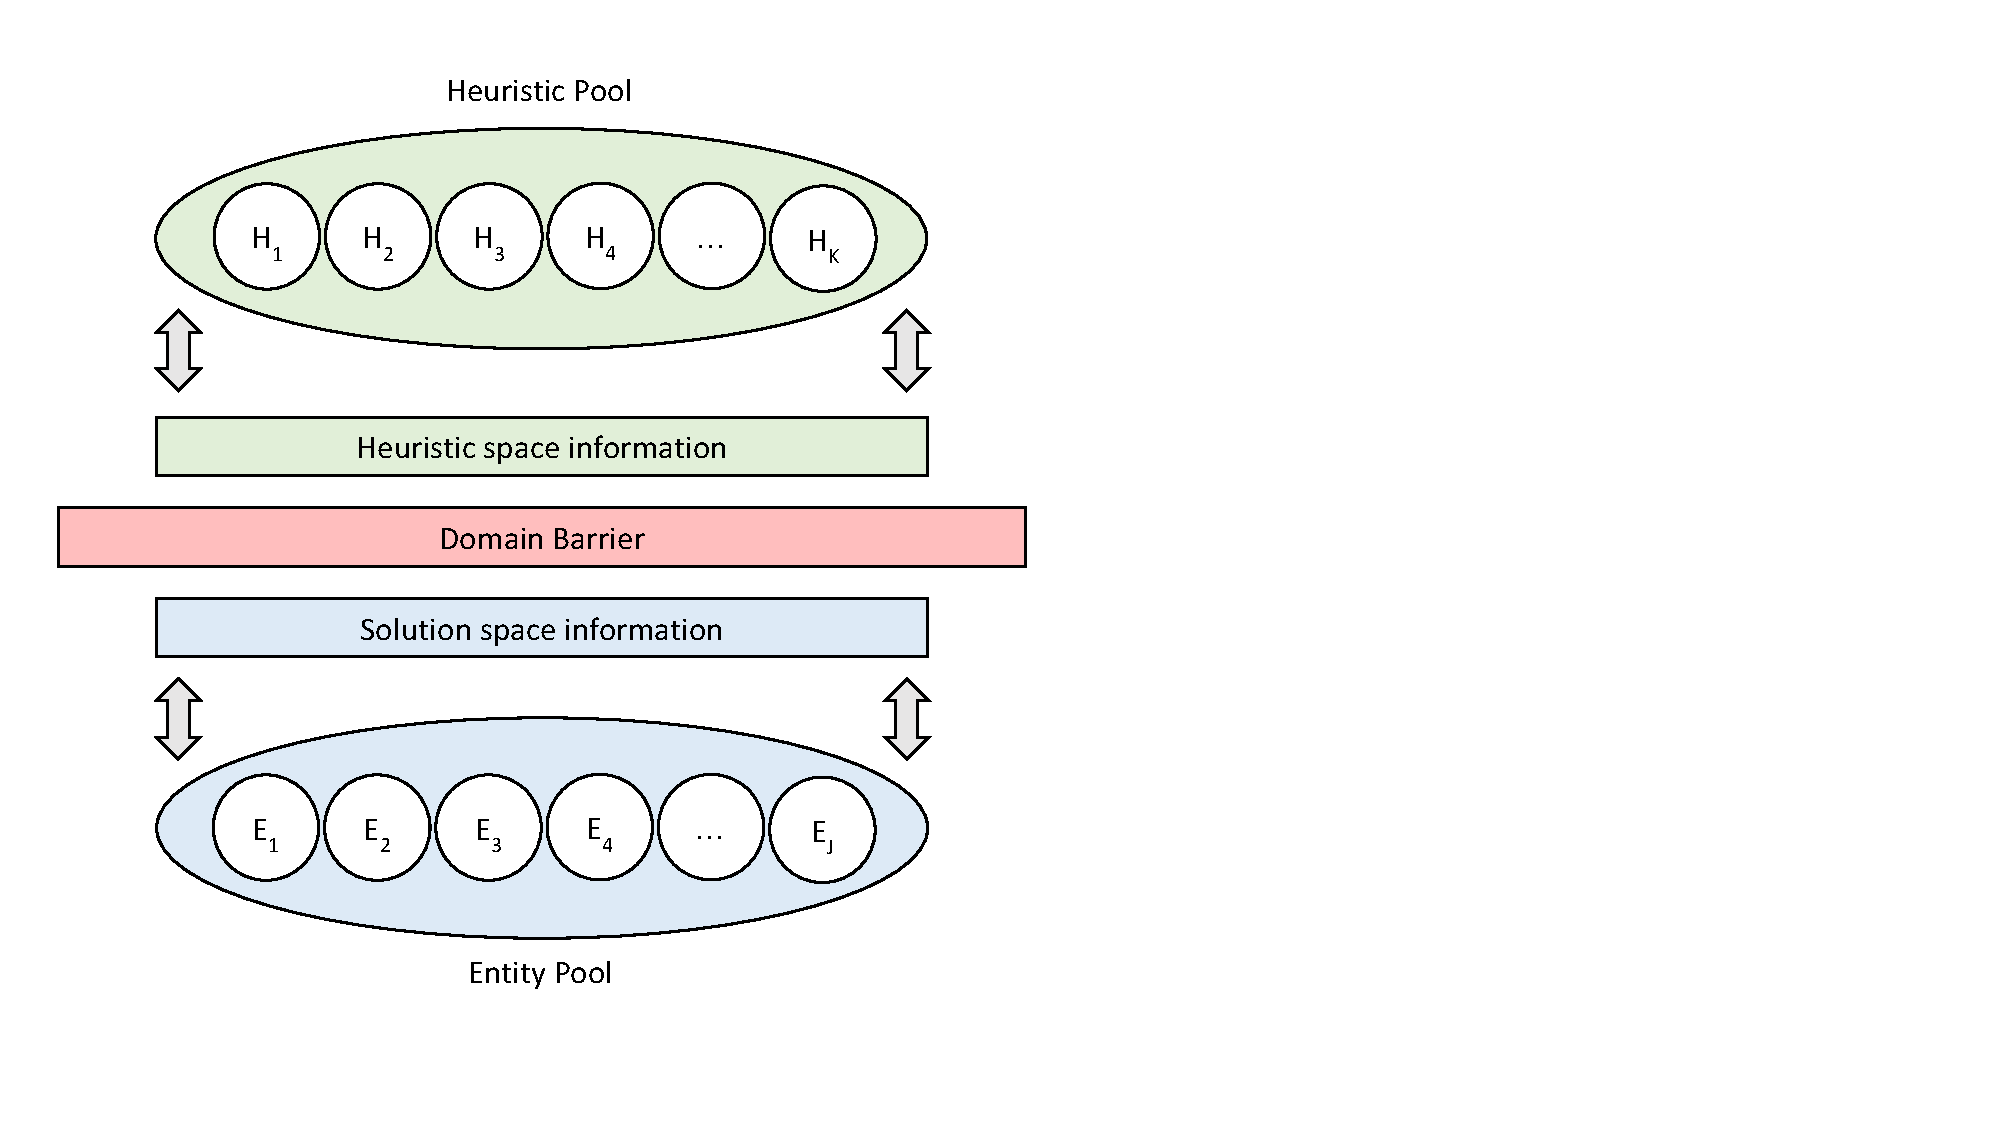
\includegraphics[width=0.65\textwidth]{images/hh_domain_barrier.pdf}
            \caption{An illustration of the domain barrier that exists as a result of the separation between the low-level \index{heuristic}heuristics and the high-level \index{heuristic}heuristic as introduced by \acp{HH}.}
            \label{fig:heuristics:hh:hh_algorithm}
      \end{centering}
\end{figure}

Figure \ref{fig:heuristics:hh:hh_algorithm} shows the separation of information that is accessible to the entity pool and heuristic pool. At a higher level abstraction, the high level heuristic implemented by \acp{HH}, do not make use of domain specific information such as an entity's position or gradient from the search space.

To summarise, \citeauthor{ref:grobler:2015}~\cite{ref:grobler:2015} highlights two fundamental ideas behind \acp{HH}. Firstly, the recognition that the process of selecting or designing efficient hybrid and/or cooperative heuristics can be regarded as a computational search problem in itself. Secondly, there is significant potential to improve search methodologies by the incorporation of learning mechanisms that can adaptively guide the search. These two fundamental ideas have inspired different types of hyper-heuristics~\cite{ref:burke:2010}.

In the general context of optimisation, many different types of \acp{HH} have been implemented and applied to many different problems. Some notable examples include the \index{simulated annealing}simulated annealing-based \acs{HH} by~\citeauthor{ref:dowsland:2007}~\cite{ref:dowsland:2007}, the \index{tabu-search}tabu-search \acs{HH} of~\citeauthor{ref:burke:2010}~\cite{ref:burke:2010}, the \index{heterogeneous meta-hyper-heuristic}heterogeneous meta-hyper-heuristic by~\citeauthor{ref:grobler:2012}~\cite{ref:grobler:2012} and work done by~\citeauthor{ref:vanderstockt:2018}~\cite{ref:vanderstockt:2018} on the analysis of selection hyper-heuristics for population-based \acp{MH} in real-valued dynamic optimization. Research on the application of \acp{HH} in the context of \acs{FFNN} training is still scarce.~\citeauthor{ref:nel:2021}~\cite{ref:nel:2021} provides the first research in this field, applying a \acs{HH} to \acs{FFNN} training. The following section provides a framework for \acs{HH} classification.


\section{Classification of Hyper-Heuristics}\label{sec:hh:classification}

\citeauthor{ref:burke:2010}~\cite{ref:burke:2010} proposed a modern classification scheme used to classify \acp{HH}. According to the proposed classification scheme, \acp{HH} are classified in two dimensions. These include the \textit{source of feedback} used during learning and the nature of the \textit{heuristic search space}. Figure \ref{fig:heuristics:hh:classification} presents the classification scheme as proposed by~\citeauthor{ref:burke:2010}~\cite{ref:burke:2010}.

\begin{figure}[htbp]
      \centering
      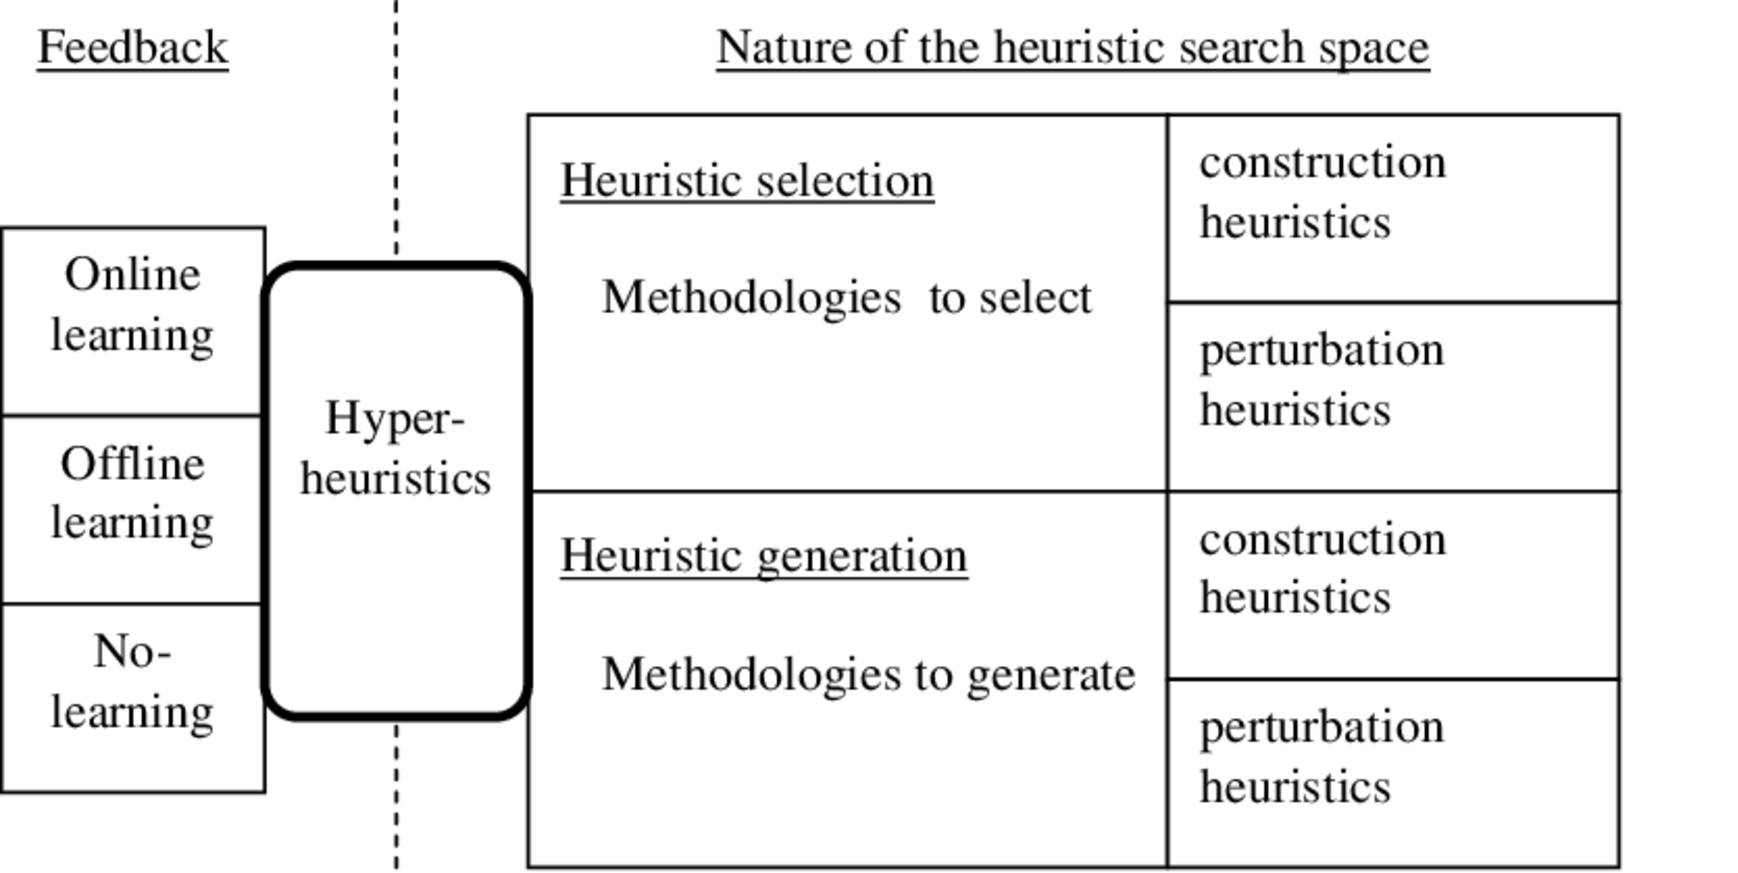
\includegraphics[width=\textwidth]{images/hh_classification.pdf}
      \caption{A classification of \acs{HH} approaches, according to two dimensions: (i) the source of feedback used during learning, and (ii) the nature of the heuristic search space.}
      \label{fig:heuristics:hh:classification}
\end{figure}

\subsection{Source of Feedback}

\acp{HH} make use of feedback from the search process to adapt and guide the search process. Some \acp{HH} implement a learning mechanism that utilises this feedback. Learning \acp{HH} can implement a form of \index{online learning}\textit{online learning} or \index{offline learning}\textit{offline learning}.

\acp{HH} that implement \index{online learning}online learning, implement a form of learning that continues to takes place while the algorithm is solving an instance of the underlying optimisation problem. Task-dependent, local properties can be used by the high-level \index{heuristic}heuristic to determine the appropriate low-level heuristic to apply at various points in the search process. Examples of \index{online learning}online learning approaches within \acp{HH} include the use of \acf{RL} and \acfp{MH} as high-level search strategies.

\acp{HH} that implement \index{offline learning}offline learning, implement a form of learning where knowledge, in the form of rules or programs, is gathered from a set of training instances and is then applied independently from the search process itself. Examples of offline learning approaches within hyper-heuristics include \textit{learning classifier systems} and \textit{case-based reasoning}.

\subsection{Heuristic Search Space}
According to the classification proposed by~\citeauthor{ref:burke:2010}~\cite{ref:burke:2010}, the second dimension of classification involves the nature of the \index{heuristic}heuristic search space. Distinction is made between \index{heuristic}heuristic \textit{selection} and heuristic \textit{generation}.

\subsubsection{Selection vs. Generation}

Selection \acp{HH} implement a high-level search mechanism that is used to determine which heuristic to apply to the underlying optimisation problem at a given point in the optimisation process. Selection mechanisms can include probabilistic approaches or high level \acfp{MH}. On the contrary, \index{heuristic}heuristic generation methodologies implement a mechanism that generate new heuristics from a pool of \textit{components} of various heuristics. Generation \acp{HH} often make use of \acfp{EA}~\cite{ref:burke:2010}.

Selection \acp{HH} consist of two components, including a low-level \index{heuristic}heuristic selection strategy and a move acceptance strategy. Low-level \index{heuristic}heuristic selection can be done in a simple, \textit{non-adaptive} way. No learning is involved in these approaches. For non-adaptive techniques, heuristic selection is based on a predefined heuristic ordering that is generated either randomly or in a ordered cycle that is repeated throughout the optimisation process~\cite{ref:cowling:2000}. As an alternative, heuristic selection may incorporate an \textit{adaptive} (\index{online learning}\textit{online learning}) mechanism, based on the probabilistic weighting of the low-level heuristics~\cite{ref:burke:2003} or some type of performance statistics~\cite{ref:cowling:2000}.

A move acceptance strategy is the mechanism by which the application of a low-level \index{heuristic}heuristic is either accepted or rejected. In general, a move is accepted or rejected based on the quality of the move and the current solution during a single point search.~\citeauthor{ref:burke:2003}~\cite{ref:burke:2003} mention that many move acceptance strategies have been explored within \acp{HH}.

Move acceptance strategies can be divided into two categories. These include \textit{deterministic} and \textit{non-deterministic} move acceptance strategies. Deterministic move acceptance strategies generate the same result for the same candidate solution(s) used for the move acceptance test. Non-deterministic move acceptance strategies can involve other parameters, such as the current time, or a sampling operation that yields possibly different outcomes when repeated for the move acceptance test~\cite{ref:burke:2003}.


\subsubsection{Construction vs. Perturbation}

Selection and generation \acp{HH} can be further classified in terms of \textit{construction} and \textit{perturbation} mechanisms. According to~\citeauthor{ref:burke:2010}~\cite{ref:burke:2010}, construction approaches build a solution incrementally. Starting with an empty solution, the goal is to intelligently select and use construction heuristics to gradually build a complete solution. As such, the \acs{HH} framework is provided with a set of pre-existing construction heuristics.

Perturbation  approaches refer to approaches that start with a complete solution, generated either randomly or using simple construction heuristics.  Perturbation heuristics try to iteratively improve the current solution. As such, the hyper-heuristic framework is provided with a set of neighbourhood structures and/or simple local searchers.


\section{Summary}\label{sec:hh:summary}

This chapter provided the reader with the necessary background information on \index{meta-learning}meta-learning and \acp{HH}. Formal definitions were given, followed by detailed discussions. A modern classification scheme for \acs{HH} as proposed by~\citeauthor{ref:burke:2010}~\cite{ref:burke:2010} was presented in detail. Distinction is made between the source of feedback information used during learning and the nature of the heuristic search space. Detailed discussions on selection and generation heuristics are provided, followed by a further classification of construction and perturbation mechanisms.

This chapter concludes the background information of \index{heuristic}heuristics in general. The following chapter aims to provide the reader with the necessary background information on statistics and probability theory.